\section{Experiments}\label{sec:experiments}
To demonstrate the use of our {\em GeoTracking} and {\em GeoRouting}
extension blocks and the behavior of our {\sc breadcrumb} router, we
used our implementations of them in the IBR-DTN core and with the Java
API and performed end-to-end experiments on the VirtualMeshTest (VMT)
channel-emulated testbed~\cite{hahn10:using, kim11:reality}.  VMT
allows us to subject Linux-based real wireless nodes with commodity
wireless hardware to emulated mobile environments.  The wireless
testbed is effectively an analog channel emulator based on an array of
programmable attenuators.  Given a desired physical arrangement of
nodes, the system computes the expected path loss between nodes and
programs the attenuators to achieve those path loss properties.  By
updating the attenuations every second, VMT can emulate a mobile
wireless environment for real wireless nodes.

We deployed our {\sc breadcrumb} router with the new {\em GeoTracking}
and {\em GeoRouting} extension blocks on the network of VMT nodes. In
addition, for each of the experiments described below, we defined one
node in the network to be a {\em sender} and another node to be a {\em
  responder}, on which we deployed our spatiotemporal trajectory
application. Using the Java IBR-DTN bridge API, we used this
application to create application-level bundles, that we sent through
our {\sc breadcrumb} router. Specifically, the {\em sender} initially
creates a probe bundle, to which it attaches a {\em GeoTracking}
extension block. The {\em sender} then sends this bundle to the {\em
  responder} using his EID as the target of routing. When the {\em
  responder} receives this bundle at the application level, it creates
a bundle with a {\em GeoRouting} tracking block. This tracking block
specifies as waypoints a subset of the locations visited by probe. The
geo-routed bundle is sent back to the sender using the constructed
{\em GeoRouting} block to direct it. We evaluate this bi-directional
communication pattern on three increasingly sophisticated mobility
scenarios.

{\bf The Ladder.} The first scenario contains thirteen nodes. Eight of
the nodes form two evenly spaces parallel lines; these form the sides
of the ladder. One node sits, stationary, at the bottom of the ladder;
another node sits, stationary, at the top of the ladder. Three nodes
repeatedly climb from the bottom of the ladder to the top and back
down. {\color{red} The sender is at the top of the ladder and the
  responder at the bottom; Figure~\ref{fig:ladder1} shows the
  trajectory of the responder's geo-routed bundle, with the target
  location waypoints from the {\em GeoRouting} extension block
  highlighted.}
\begin{figure}
\begin{center}
\begin{tikzpicture}
\begin{axis}[legend pos=south east]
\addplot+[only marks,color=black,mark=*,mark size=0.2pt] 
	table[x=x,y=y] {../data/ladder/pgy.txt};
%\addplot[only marks,color=red,mark=x] 
%	table[x=x,y=y] {../data/ladder/pgy_2.txt};
\legend{Bundle Trajectory}
\end{axis}
\end{tikzpicture}
\end{center}
\vspace{-.75cm}
\caption{Ladder Experiment 1}\label{fig:ladder1}
\vspace{-.5cm}
\end{figure}

{\bf Crop Circles.} In our second set of experiments, we created grids
of nodes that move continuously in circles in either a clockwise or
counter clockwise patter. The simple crop circles scenario consists of
six nodes arranged as shown in Figure~\ref{fig:cropcircle1}; the
complex crop circles scenario consists of 18 nodes in six rows of
three nodes each. The sender is the node in the lower left corner; the
responder is the node in the upper right corner.
\begin{figure}
\vspace{-.2cm}
\begin{center}
%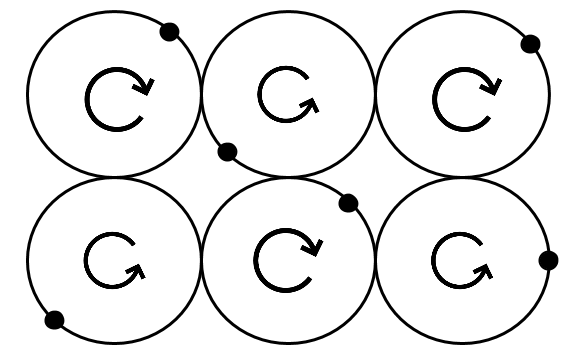
\includegraphics[width=\columnwidth+.5]{figures/cropcircle1.png}
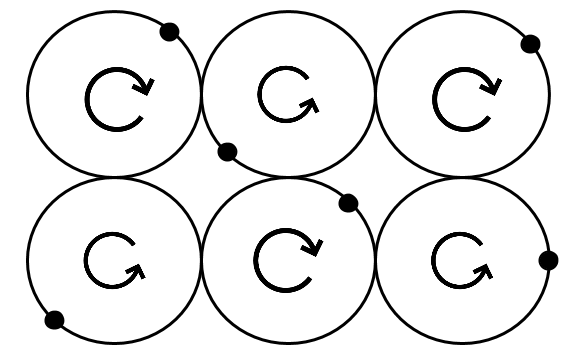
\includegraphics[width=3in]{figures/cropcircle1.png}
\end{center}
\vspace{-.75cm}
\caption{Simple crop circles mobility scenario}\label{fig:cropcircle1}
\vspace{-.25cm}
\end{figure}

\begin{figure}
%\vspace{-.2cm}
\begin{center}
\begin{tikzpicture}
\begin{axis}[legend pos=south east]
\addplot+[only marks,color=blue,mark=*,mark size=0.2pt] 
	table[x=x,y=y] {../data/cropcircles_2_3/exp1/exp1_to/crop1_to.txt};
\addplot+[only marks,color=green,mark=*,mark size=0.2pt] 
	table[x=x,y=y] {../data/cropcircles_2_3/exp1/exp1_from/crop1_from.txt};
\addplot[color=red,mark=triangle*,mark size=1pt] 
	table[x=x,y=y] {../data/cropcircles_2_3/exp1/exp1_from/exp1_from-hop-0.dat};
\addplot[color=red,mark=triangle*,mark size=1pt] 
	table[x=x,y=y] {../data/cropcircles_2_3/exp1/exp1_from/exp1_from-hop-1.dat};
%	table[x=x,y=y] {../data/ladder/pgy_2.txt};
\legend{Tracking bundle, Routing bundle}
\end{axis}
\end{tikzpicture}
\end{center}
\vspace{-.4cm}
\caption{Crop Circles Experiment 1}\label{fig:exp1}
\vspace{-.35cm}
\end{figure}

{\color{red}Here's where the plots with the crop circles go.}

{\bf The Maze.} Our final experiments mirror the motivating scenario
of the prisoner in the maze. The maze consists of a series of
connected hallways, each patrolled by a single guard who moves back
and forth along hallway. Our maze is shown in
Figure~\ref{fig:maze}. {\color{red}The sender (i.e., the prisoner) is ???? and the
  responder (i.e., the rescuer) is ???.}
\begin{figure}
\begin{center}
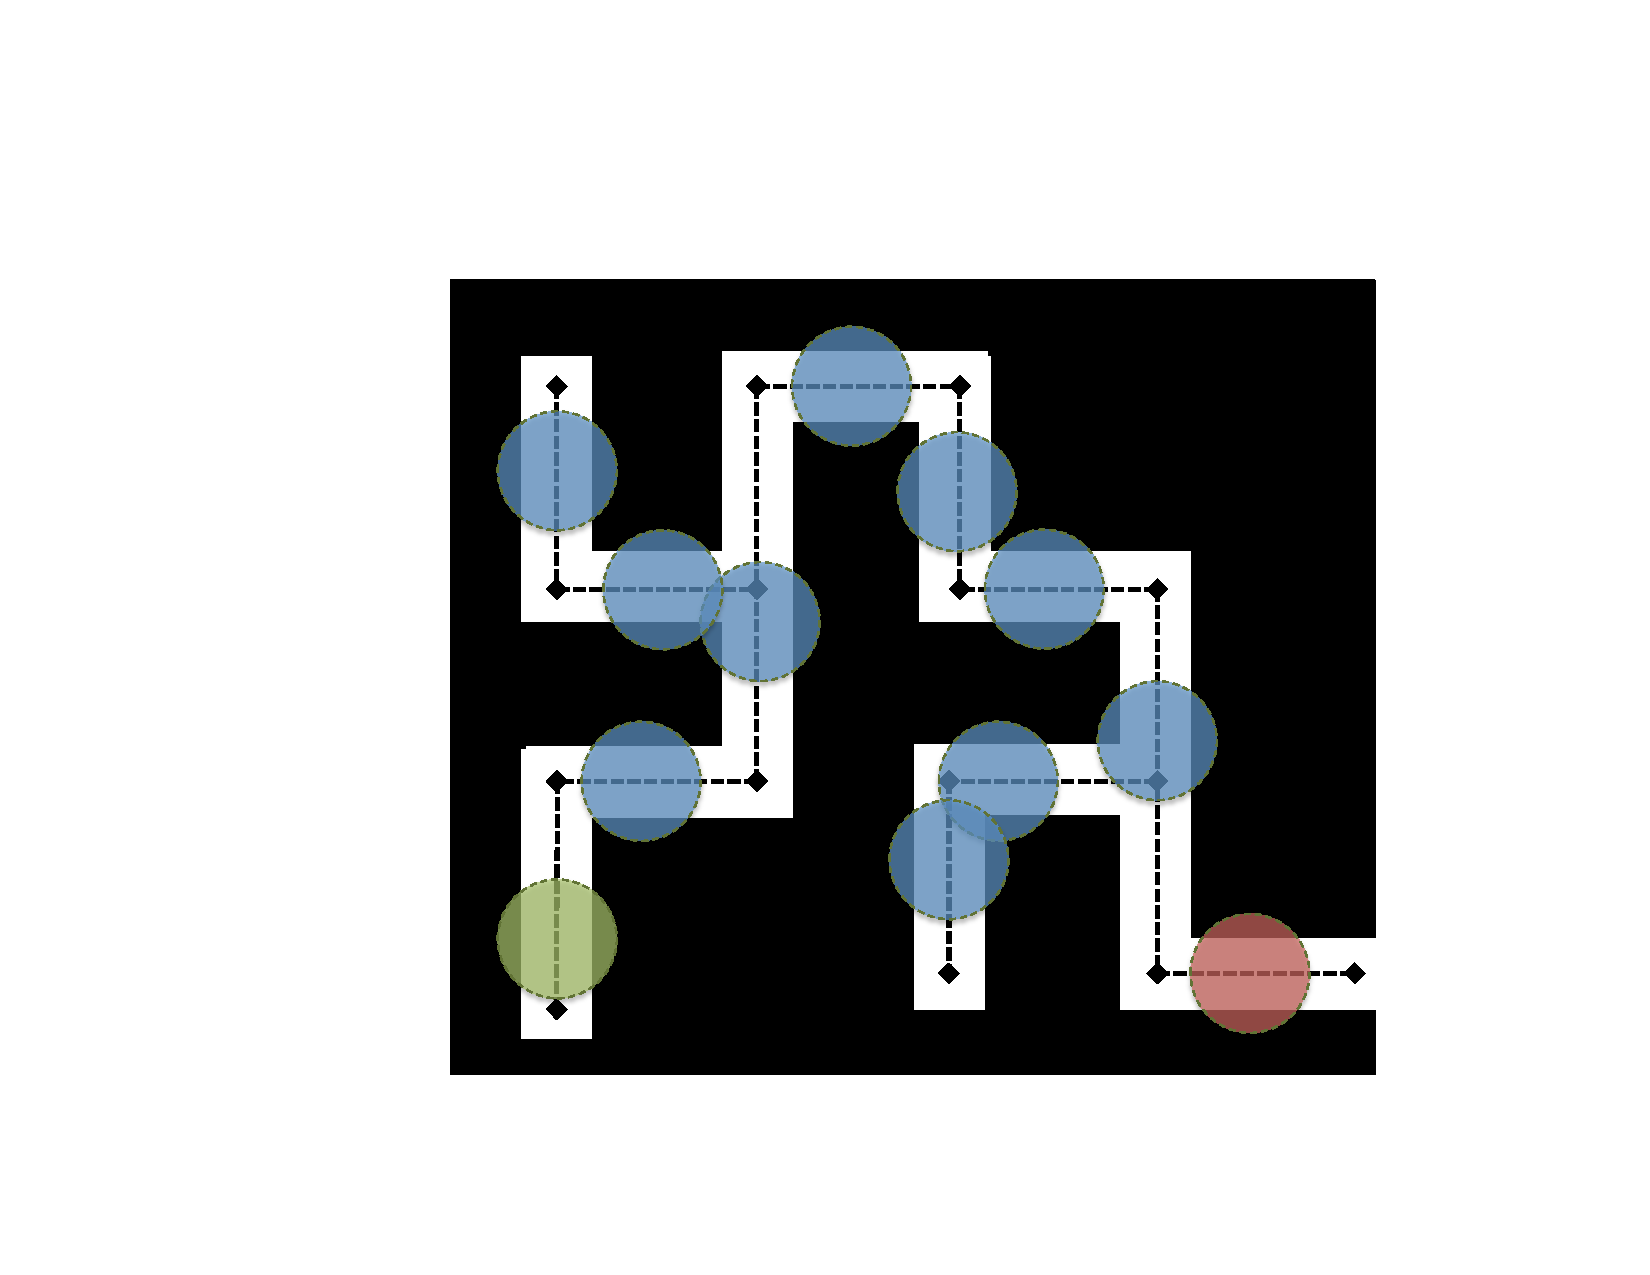
\includegraphics[width=.9\columnwidth]{figures/newMaze.pdf}
\end{center}
\vspace{-.75cm}
\caption{Maze mobility scenario}
\label{fig:maze}
\vspace{-.5cm}
\end{figure}

{\color{red}Here's where the plots with the maze go.}